\chapter{Fake rate of photon detection}

In chapter~\ref{ch:snr} we measured the signal to noise ratio after filtering.
The point of using the SNR is expressing the signal height relative to the
width of the noise distribution, because the threshold required to reject noise
with a fixed probability is proportional to that scale. So it is convenient to
express the threshold relative to the same scale, and check it is less than the
SNR so that signals are not selected away.

Even assuming that the noise is gaussian, the probability that a random
fluctuation gets over the threshold is not given simply by computing the
survival function (i.e.\ the integral to $+\infty$) of the gaussian
distribution at the threshold.

More precisely, the probability that any given sample is above the threshold is
given by such integral. What we need, however, is the \emph{rate} of threshold
\emph{crossings}. The noise is not white, but even if it was, after applying
the filter, which combines linearly many input samples for each output sample,
the waveform is autocorrelated at least up to the length of the filter.
Intuitively, if a smooth function crosses a threshold, it takes some time to go
down before it can cross the threshold again.

Since the first stage filtering procedure that will be used in DarkSide20k is
not decided at this point, for brevity we will just see how to compute the
threshold crossing rate of the noise, called fake rate, for a specific example
filter, and check that it works. The method can then be applied to any filter
of choice.

\section{Theory}

We expect the noise to be gaussian. Even if it wasn't, when filtering many
samples are linearly combined, and the sum of random variables tends to have a
gaussian distribution independently of the initial one, so we assume
gaussianity.

\subsection{From the continuous case}

We have a discrete sequence of samples. The continuous equivalent is a Gaussian
process. We can expect the discrete case to be equivalent to the continuous
case if the autocorrelation time is larger enough than the sampling step, which
should hold from the consideration above.

Also, even though the values are initially discrete too, after filtering the
possible non integer values between two consecutive integers are at least the
length of the filter (think about an average). So we take the formula for the
continuous case and adapt it.

The mean number of threshold upcrossings $r$ in the interval $(0,1)$ by a
zero-mean stationary and appropriately smooth Gaussian process is given by
\cite[81]{rasmussen2006}
%
\begin{equation}
    r = \sqrt{-\frac{k''(0)}{2\pi}} \operatorname{gauss}(u;0,\sigma),
\end{equation}
%
where $u$ is the threshold, $\sigma$ the noise standard deviation (the RMS),
$\operatorname{gauss}(x;\mu,\sigma)$ a Gaussian probability density on $x$ with
mean $\mu$ and standard deviation $\sigma$, and $k$ the autocovariance
function, i.e.\ $k(x) = \operatorname{Cov}[f(t), f(t+x)]$ for any $t$ (for
example, $k(0) = \sigma^2$), where $f(t)$ is the continuous waveform.

We have to map the second derivative of the autocovariance function to a
discrete equivalent. We first do a manipulation in the continuous realm. Since
the covariance operator is an integral, it commutes with derivation:
%
\begin{align}
    k''(x)
    &= \frac{\partial^2}{\partial x^2} \operatorname{Cov}[f(t), f(t+x)] = \\
    &= \operatorname{Cov}[f(t), f''(t+x)],
\end{align}
%
thus $k''(0) = \operatorname{Cov}[f(t), f''(t)]$. We estimate the second
derivative with a finite difference:
%
\begin{align}
    f(t \pm \Delta t)
    &= f(t) \pm f'(t) \Delta t + \frac12 f''(t) \Delta t^2 + O(\Delta t^3)
    \rightarrow \\
    \rightarrow f''(t) \Delta t^2 &=
    f(t + \Delta t) + f(t - \Delta t) - 2 f(t) + O(\Delta t^3).
\end{align}
%
Choosing $\Delta t = 1/f_s$, where $f_s$ is the sampling frequency, and calling
$y_i = f(t_0 + i\Delta t)$ the samples, we have:
\begin{align}
    k''(0) &\mapsto f_s^2 k_2, \\
    k_2 &\equiv \operatorname{Cov}[y_i, y_{i+1}+y_{i-1}-2y_i], \label{eq:k2} \\
    r &= f_s \sqrt{-\frac{k_2}{2\pi}} \operatorname{gauss}(u;0,\sigma).
    \label{eq:rcont}
\end{align}
%
The reader can check that discretizing directly $k''(0)$ yields the same result.

The covariance in equation~\ref{eq:k2} can be estimated with the sample
covariance on a filtered waveform array~$\mathbf y$.

\subsection{Direct discrete derivation}

Since the formula we derived is approximate, as a cross check we derive another
approximate one following a different path.

A threshold crossing happens when a sample is below the threshold and the next
one is above: $y_i \leq u$, $y_{i+1} > u$. Fix $i=0$ and let $p(y_0,y_1)$ be the
joint distribution of the two samples. The probability of crossing at any given
point then is
%
\begin{equation}
    P =
    \int_{-\infty}^u \mathrm d y_0\,
    \int_u^\infty \mathrm d y_1\,
    p(y_0, y_1).
    \label{eq:crossingprob}
\end{equation}

In general we can not obtain the crossing rate just by multiplying $P$ by the
sampling frequency because of correlations. However in practice we are
interested in low crossing rates, on the order of~\SI{10}{cps}, to be compared
to the sampling frequency~\SI{125}{MSa/s}. If the typical time between
crossings is much longer than the autocorrelation time, then we can ignore
correlations. Thus the crossing rate is $r = f_s P$.

The integrand in equation~\ref{eq:crossingprob} is a bivariate gaussian
distribution, which explicitly is
%
\begin{equation}
    p(y_0,y_1) =
    \frac 1 {2\pi \sqrt{\sigma^4 - c^2}}
    \exp \left(
    \frac 1 2
    \begin{pmatrix}
        y_0 & y_1
    \end{pmatrix}
    \begin{pmatrix}
        \sigma^2 & c \\
        c & \sigma^2
    \end{pmatrix}^{-1}
    \begin{pmatrix}
        y_0 \\ y_1
    \end{pmatrix}
    \right),
\end{equation}
%
where $c = \operatorname{Cov}[y_0, y_1]$.

We don't know how to the integral analytically, so we break down the joint
distribution as $p(y_0,y_1) = p(y_1|y_0) p(y_0)$ and discretize the integral
over $y_0$:
%
\begin{align}
    p(y_0) &= \operatorname{gauss}(y_0; 0, \sigma), \\
    p(y_1|y_0) &= \frac {p(y_0, y_1)} {p(y_0)}
    = \operatorname{gauss} \left(
        y_1; \frac c {\sigma^2} y_0, \sqrt{\sigma^2 - \frac {c^2} {\sigma^2}}
    \right), \\
    P &\approx
    \sum_{k=0}^{N-1} \Delta u\, p(y_0(k,u,\Delta u))
    \int_u^\infty \mathrm d y_1\, p(y_1|y_0(k,u,\Delta u)), \label{eq:rdisc} \\
    y_0(k,u,\Delta u) &\equiv u - k \Delta u.
\end{align}

The integral on $y_1$ can be computed using the error function. $\Delta u$
should be chosen small compared to $\sigma$, while $N$ large relative to
$\sigma / \Delta u$.

In figure~\ref{fig:crossingprob} we compare formula~\eqref{eq:rcont} (with $f_s
= 1$) with $P$ and with the Gaussian survival function. To make the comparison
we have to use a $k_2$ that matches $c$:
%
\begin{align}
    k_2 &= \operatorname{Cov}[y_i, y_{i+1}+y_{i-1}-2y_i] = \notag \\
    &= \operatorname{Cov}[y_i,y_{i+1}]
    + \operatorname{Cov}[y_i,y_{i-1}]
    - 2 \operatorname{Cov}[y_i,y_i] = \notag \\
    &= 2 (c - \sigma^2).
\end{align}
%
We use $\sigma=1$, $c = \SI{99}\%$, $\Delta u = 1/100$, $N=500$ (we decreased
$\Delta u$ until convergence). We see that our derivation and the formula
for Gaussian processes agree very well, while differing visibly from the
survival function. We will henceforth use the continuous formula for its
simplicity.

\begin{figure}
    \hspace{0.00\textwidth}
    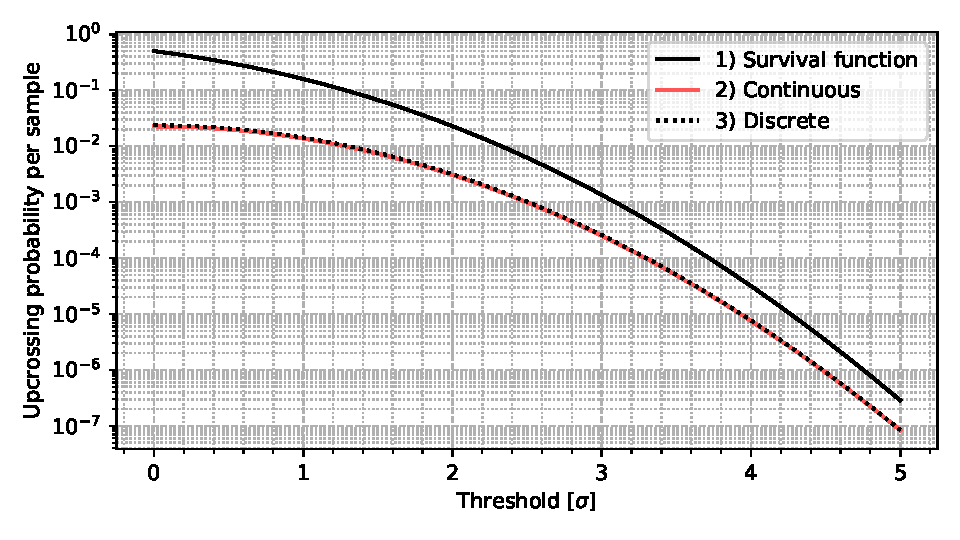
\includegraphics[width=1.00\textwidth]{figcrossingprob}

    \caption{\label{fig:crossingprob} The threshold upcrossing rate expressed
    as per-sample crossing probability (i.e.\ the rate if the sampling
    frequency is~1) for an autocorrelated Gaussian waveform, estimated using
    three formulae: 1) the probability for a single sample to be higher than
    the threshold, 2) a formula for continuous processes
    (equation~\ref{eq:rcont}), 3) an approximation of the discrete case
    (equation~\ref{eq:rdisc}).}
    
\end{figure}

\subsection{Dead time}

The part of the data acquisition system (DAQ) that will look for threshold
crossings are the digitizers. A digitizer can not do complicated processing, so
when the threshold is crossed, a fixed slice of waveform is sent to the front
end processing (FEP) for further analysis (identify multiple signals, locate
them precisely, use a better filter, etc.). So we are not interested in
threshold crossings that happen close to a previous crossing.

This means that we have a dead time $T$. We arbitrarily decide to use a
non-restartable dead time, i.e.\ a crossing that happens within $T$ of a
previous one is ignored only if the latter has not been ignored itself.

Assuming that the crossings are a Poisson process, the formula to correct a
rate $R$ for the effect of the dead time is \cite[120]{knoll2000}:
%
\begin{equation}
    R \mapsto \frac R {1 - RT}.
\end{equation}

The crossings of a Gaussian process are not in general a Poisson process. We
just need one counterexample to show this. Consider the process with
autocovariance function $k(x)=\cos(x)$. This is positive definite because it is
a linear combination of external products: $\cos(x-y) = \cos x \cos y + \sin x
\sin y$. Since $\cos$ is orthogonal to $\sin$, they are the eigenfunctions, so
a realization of the process is a random linear combination of harmonic
functions, which means that it is a shifted cosine, so the crossings are
exactly periodic.

However, in practice we expect that there will just be a ``repulsion'' or
``attraction'' of crossings within the scale of the autocorrelation time, so
for low crossing rate the formula should work.

\section{Test}

We want to test formula~\eqref{eq:rcont} on actual electrical noise.

\subsection{Data}

We will use the Proto0 run 886, a baseline acquisition. Tiles 53, 57 and 59
(used in Proto0) will be also studied with LNGS data. Tile~15 just with LNGS.
The LNGS data files are:
%
\begin{verbatim}
FBK/NUV/MB2-LF-3x/NUV-LF_3x_53/nuvhd_lf_3x_tile53_77K_64V_6VoV_1.wav
FBK/NUV/MB2-LF-3x/NUV-LF_3x_53/nuvhd_lf_3x_tile53_77K_66V_7VoV_1.wav
FBK/NUV/MB2-LF-3x/NUV-LF_3x_57/nuvhd_lf_3x_tile57_77K_64V_6VoV_1.wav
FBK/NUV/MB2-LF-3x/NUV-LF_3x_59/nuvhd_lf_3x_tile59_77K_64V_6VoV_1.wav
LFOUNDRY/pre-production-test/TILE_15/LF_TILE15_77K_55V_0VoV_1.wav
LFOUNDRY/pre-production-test/TILE_15/LF_TILE15_77K_59V_2VoV_1.wav
LFOUNDRY/pre-production-test/TILE_15/LF_TILE15_77K_63V_4VoV_1.wav
LFOUNDRY/pre-production-test/TILE_15/LF_TILE15_77K_67V_6VoV_1.wav
LFOUNDRY/pre-production-test/TILE_15/LF_TILE15_77K_71V_8VoV_1.wav
LFOUNDRY/pre-production-test/TILE_15/LF_TILE15_77K_73V_9VoV_1.wav
\end{verbatim}

\marginpar{Expand and adapt this paragraph after chapter 3 is done.}

The Proto0 data is without signals so we use it as it is. For the LNGS data
we take the pre-trigger part of the events, and ignore events where any
pre-trigger sample is less than~750 (860 for tile~15).

We plot the time-value histogram of the data for tile 53 in Proto0 and LNGS
(figure~\ref{fig:hist2dtile53}), for tile 15 at maximum overvoltage, and for
tiles 57 and 59 (figure~\ref{fig:hist2dtile155759}).

\marginpar{No need for more explanations of the time-value histograms since
there will be some of them in chapter 3.}

\begin{figure}
    
    \mbox{
    \hspace{-0.20\textwidth}
    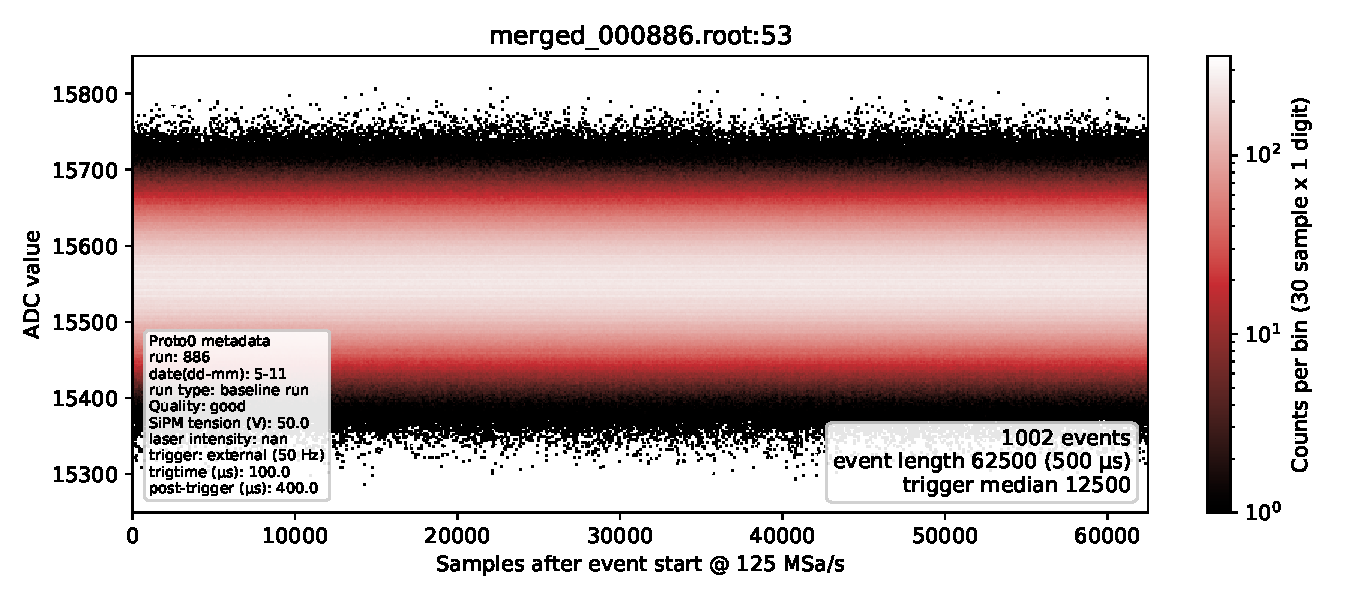
\includegraphics[width=1.41\textwidth]{fighist2dtile53-0}
    }
    \mbox{
    \hspace{-0.20\textwidth}
    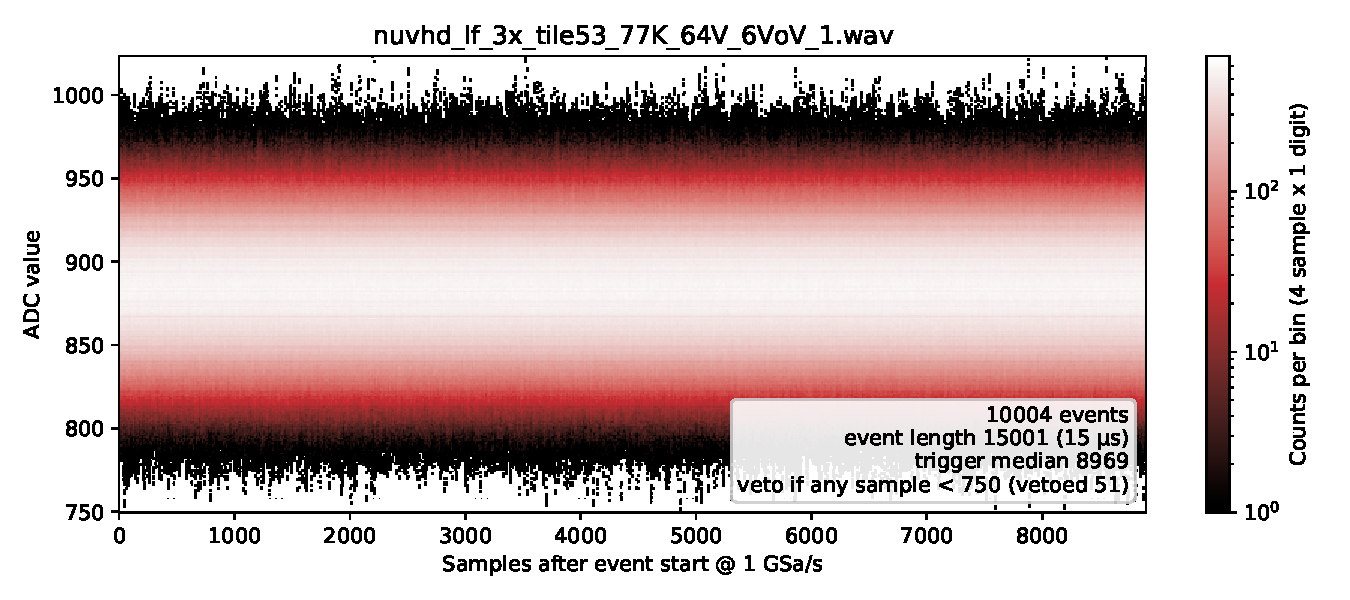
\includegraphics[width=1.41\textwidth]{fighist2dtile53-1}
    }
    \mbox{
    \hspace{-0.20\textwidth}
    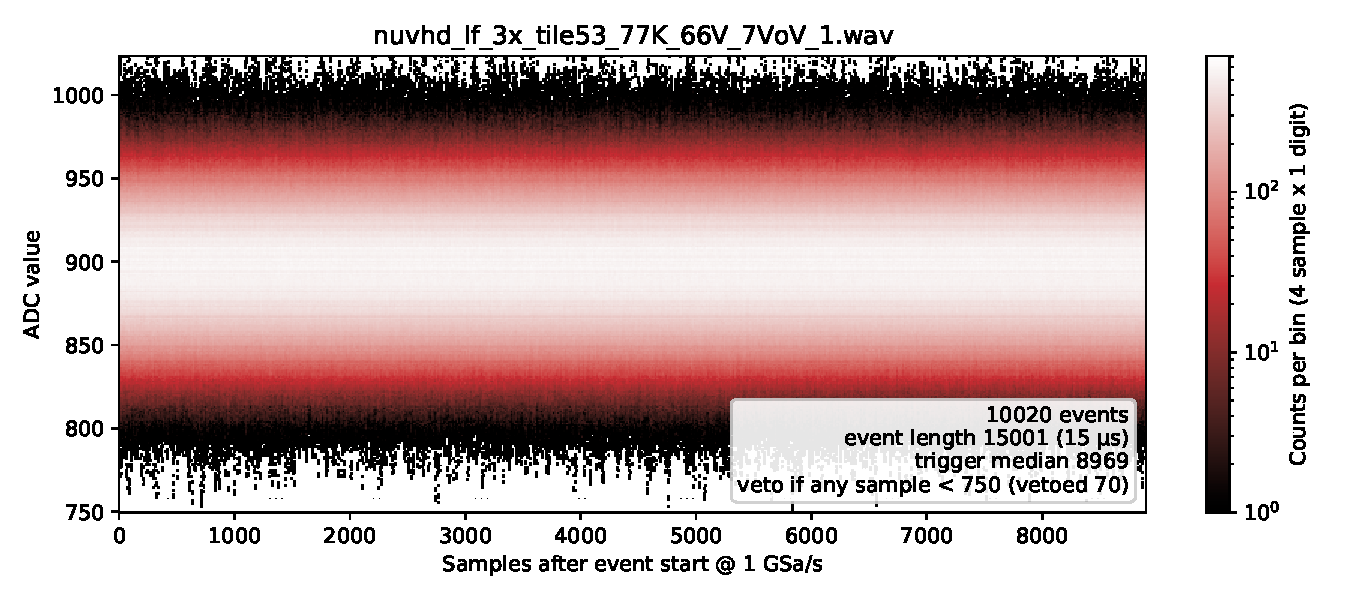
\includegraphics[width=1.41\textwidth]{fighist2dtile53-2}
    }
    
    \figcaption{hist2dtile53}{Time-value histograms of tile 53 noise in Proto0
    with a baseline acquisition, and in LNGS pre-trigger at overvoltage \SI6V
    and \SI7V.}
    
\end{figure}

\begin{figure}
    
    \mbox{
    \hspace{-0.20\textwidth}
    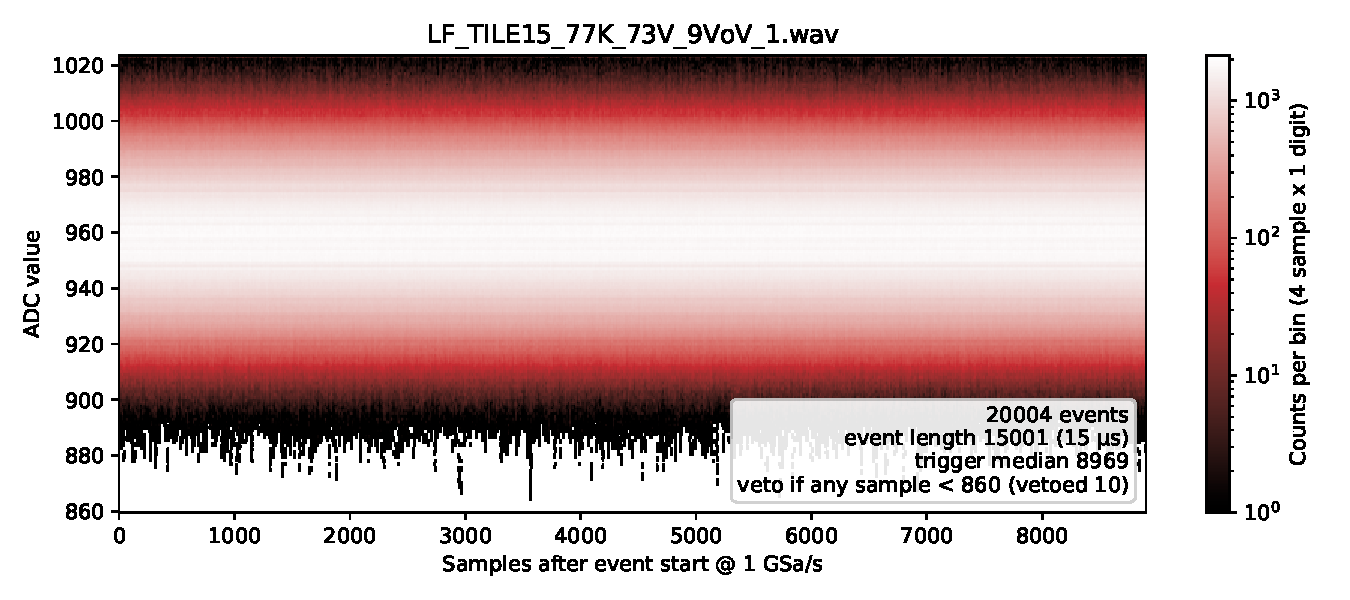
\includegraphics[width=1.41\textwidth]{fighist2dtile155759-0}
    }
    \mbox{
    \hspace{-0.20\textwidth}
    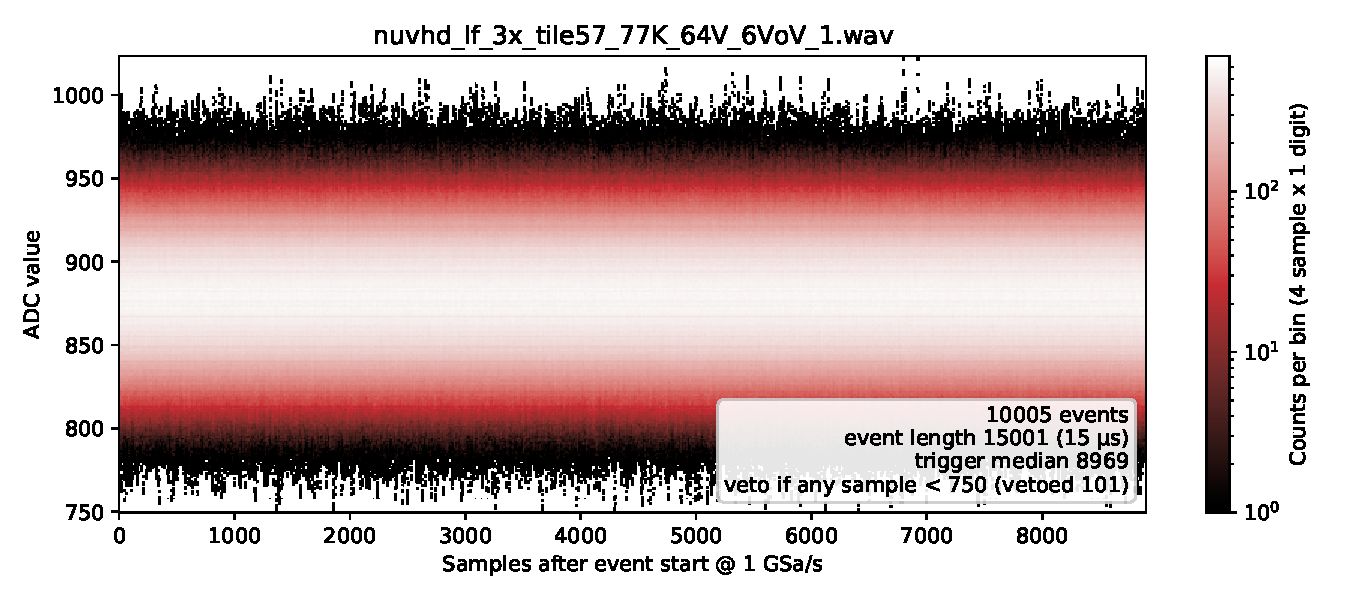
\includegraphics[width=1.41\textwidth]{fighist2dtile155759-1}
    }
    \mbox{
    \hspace{-0.20\textwidth}
    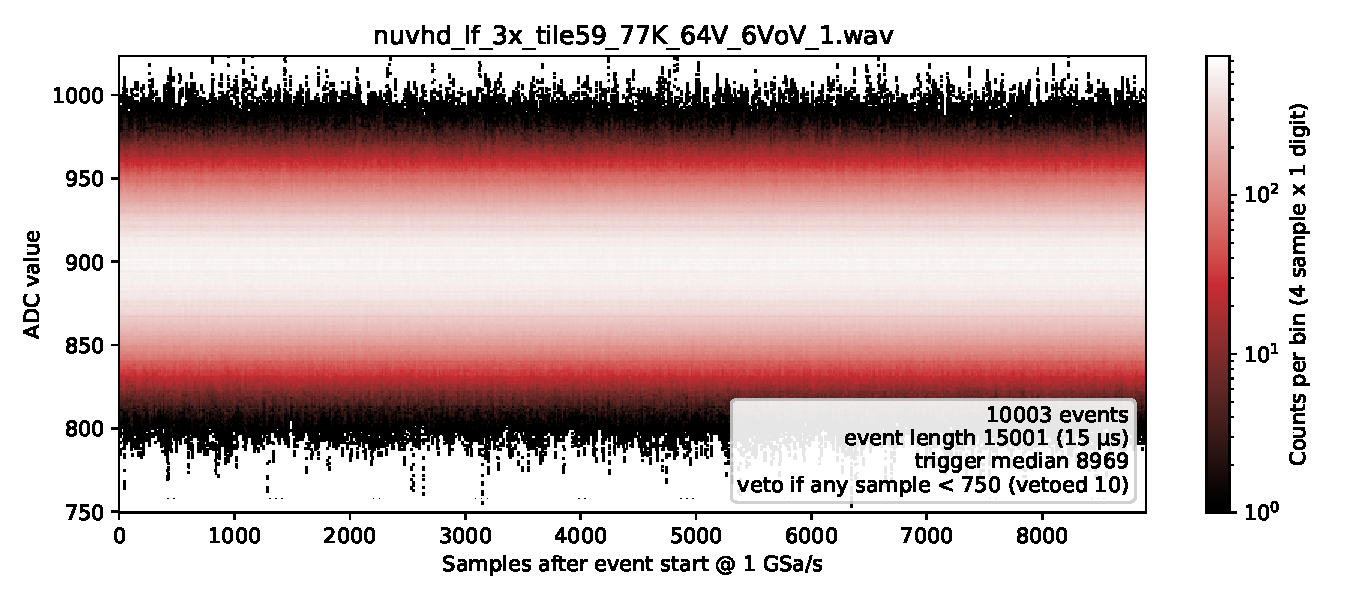
\includegraphics[width=1.41\textwidth]{fighist2dtile155759-2}
    }

    \figcaption{hist2dtile155759}{Time-value histograms of tiles 15, 57 and 59
    noise in LNGS data.}
    
\end{figure}

\subsection{Filter}

We filter using a \SI1{\micro s} moving average with \SI1{\micro s} of baseline
and \SI1{\micro s} of dead time, without delay between the baseline and the
signal averages. In figure~\ref{fig:sqfilt} we show an example filtered
waveform and the filter shape.

\begin{figure}

    \hspace{-0.20\textwidth}
    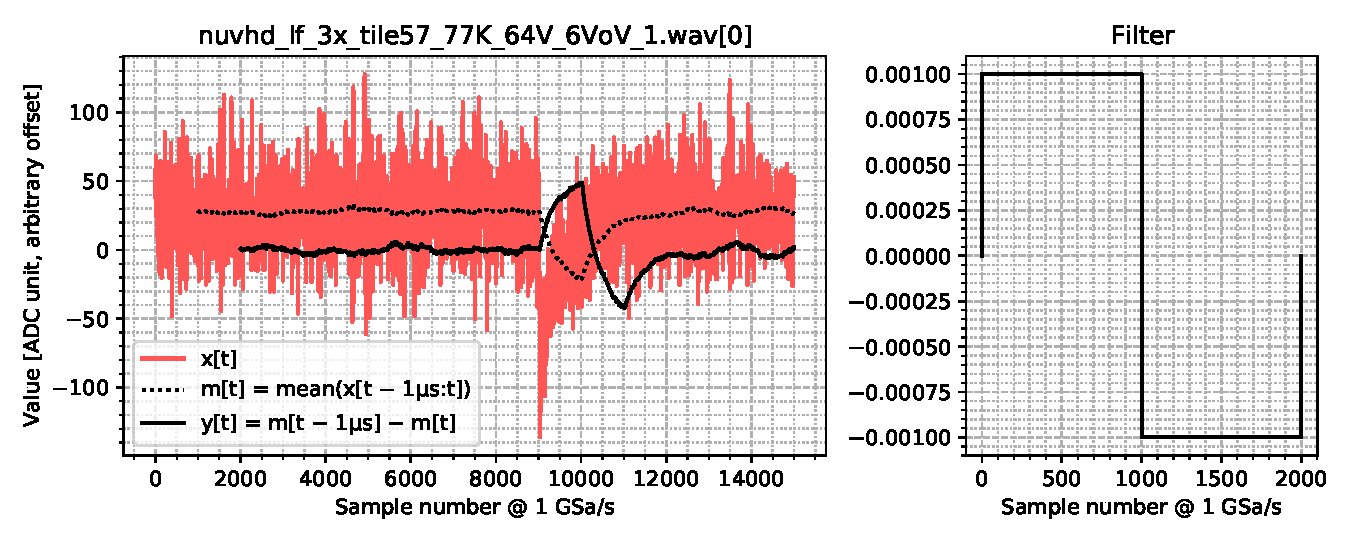
\includegraphics[width=1.41\textwidth]{figsqfilt}

    \figcaption{sqfilt}{A filtered waveform. The computation is split into a
    moving average $m$ (dotted line) and its finite difference $y$ (solid black
    line). The right plot shows the overall filter shape. (We use an event with
    a signal just to see how the filter behaves, the analysis is done on noise
    only.)}

\end{figure}

From chapters~\ref{ch:snr} and~\ref{ch:timeres} we know this is not the optimal
filter by SNR neither by temporal resolution. However since we don't know which
filter will be used it is appropriate to make a conservative choice.

Since on LNGS data the events are short compared to the filter length
(\SI9{\micro s} vs. \SI2{\micro s}), we need to take into account boundary
effects. The output length of the filtered waveform is $(\text{initial length})
- \SI2{\micro s} + \SI1{sample}$; to compute the rate we have to divide by this
quantity instead of the initial waveform length.

The dead time does not play nicely with borders, because a hypothetical unseen
crossing within \SI1{\micro s} before the event start could kill a crossing in
the event. Moreover, at low thresholds, the first crossing will happen
almost immediately, and again immediately after the dead time ends, thus the
number of crossings per event is quantized.

A complete solution to these problems would be to avoid counting the crossings
which happen within \SI1{\micro s} after the event start (although they are
detected and do project a dead time on the following ones), and in the
remaining region further select a subregion which is \SI1{\micro s} shorter but
has a uniformly random starting position.

However we care only about low rates, and at low rate the dead time boundary
effects are negligible, so we will keep the whole filtered region.

\subsection{Algorithm}



\subsection{Results}
